% !TeX spellcheck = en_US
% PAKETE UND DOKUMENTKONFIGURATION
\documentclass[11pt, a4paper]{article}

% Encoding für Umlaute
\usepackage[utf8]{inputenc}
\usepackage[T1]{fontenc}

% Silbentrennung
\usepackage[english]{babel}

% erweiterte Matheumgebungen und Formelnummer mit Sectionnummer
\usepackage{amsmath}
\numberwithin{equation}{section}

% Braket Notation
\usepackage{braket}
\usepackage{isotope}
\usepackage[version=4]{mhchem}
\usepackage{tensor}
\usepackage{slashed}

% zusätzliche mathematische Schriftarten
\usepackage{amsfonts}

% verschiedene mathematische Symbole
\usepackage{amssymb}

% sidewaysfrac
\usepackage{xfrac}

% Einheiten setzen z.B. \SI{10}{\kilo\gram\meter\per\second\squared}
% Fehler: \SI{10 +- 0,2e-4}{\metre}
\usepackage{siunitx}
\sisetup{
  output-decimal-marker={.},
  separate-uncertainty
}

% Einheitendefinitionen
\DeclareSIUnit{\skt}{Skt.}
\DeclareSIUnit{\gauss}{G}
\DeclareSIUnit{\division}{div.}
\DeclareSIUnit{\Kanal}{Kanal}

% Operatordefinitionen
\DeclareMathOperator{\erf}{erf}

% Makros
\newcommand\dinf[1]{ \,\mathrm{d}#1 }
\newcommand\deriv[2] { \frac{\mathrm{d} #1}{\mathrm{d} #2} }

% Randbreiten
\usepackage[left=3.5cm,right=3.5cm,top=3cm,bottom=3cm,twoside]{geometry}

% Bilder einfügen
\usepackage{graphicx}
\usepackage[percent]{overpic}

% Textfarbe
\usepackage{color}

% Verweise innerhalb des Dokuments
\usepackage{hyperref}
\hypersetup{
	colorlinks = true,
	allcolors = {black}
}

% bessere Tabellenlayouts
\usepackage{booktabs}
\usepackage{multirow}
\usepackage{multicol}

% Seitenlayout (Kopfzeile)
\usepackage{fancyhdr}

% Float Barriers
\usepackage{placeins}

% Pakete für gedrehte Subfigures
\usepackage{caption}
\usepackage{subcaption}
\usepackage{rotating}
\usepackage{capt-of}

% Paket für textumflossene Abbildungen und Tabellen
\usepackage{wrapfig}

\usepackage{float}

% Caption-Setup
\captionsetup{font={small}}
\renewcommand{\thefigure}{\thesection.\arabic{figure}}
\renewcommand{\thesubfigure}{\alph{subfigure}}
\renewcommand{\thetable}{\thesection.\arabic{table}}
\renewcommand{\thesubtable}{\alph{subtable}}

% Manuelle Silbentrennung
\hyphenation{Sekundär-elek-tronen-verviel-facher}

% Tiefe des Inhaltsverzeichnisses (Level: 1 sections, 2 subsections,
% 3 subsubsections)
\setcounter{tocdepth}{3}

% FANCYHDR SETUP
\pagestyle{fancy}
\fancyhead[EL,OR]{\thepage}
\fancyhead[ER]{\leftmark}
\fancyhead[OL]{\rightmark}
\setlength{\headheight}{13.6pt}

\renewcommand{\sectionmark}[1]{
\markboth{\thesection{} #1}{\thesection{} #1}
}
\renewcommand{\subsectionmark}[1]{
\markright{\thesubsection{} #1}
}

\newcommand{\korr}[1]{{\color{red}(#1)}}

% DOKUMENTINFORMATIONEN
\title{E213 \\ Analysis of Decays of Heavy Vector Boson Z$_0$}

\author{Christopher Deutsch\footnote{christopher.deutsch@uni-bonn.de} \and Christian Bespin\footnote{christian.bespin@uni-bonn.de}}

\date{\today}

\begin{document}

\begin{titlepage}

\maketitle

% DURCHFÜHRUNGSDATUM UND TUTOR
\begin{center}
\begin{tabular}{l r}
Performed: & April 20 \& 21, 2016 \\
Group: & P8 \\
Tutor: & David Hohn
\end{tabular}
\end{center}

% ZUSAMMENFASSUNG
\begin{abstract}
	\noindent 
\end{abstract}

\end{titlepage}

% INHALTSVERZEICHNIS
\tableofcontents
% Neue Seite nach TOC
\newpage

% INHALT VERSUCHSPROTOKOLL
\section{Introduction}



\section{Theoretical Background}

In the following chapter a brief overview of the knowledge needed to perform the lab experiment will be presented.

\subsection{Standard Model of Elementary Particle Physics}

The Standard Model describes the elementary particles and their interactions, excluding gravitation.
In the Standard Model particles can be grouped by their properties into quarks, leptons and interaction particles.
While quarks and leptons are fermions, the interaction particles are (gauge) bosons.
Quarks have fractional charge of $+2/3$ or $-1/3$ and leptons are either charged (with charge $\pm1$ for electron, muon and tau) or uncharged (neutrinos).
Interaction particles can also be charged (W~boson) or uncharged (photon, gluon, Z~boson).
\begin{figure}[h]
	\centering
	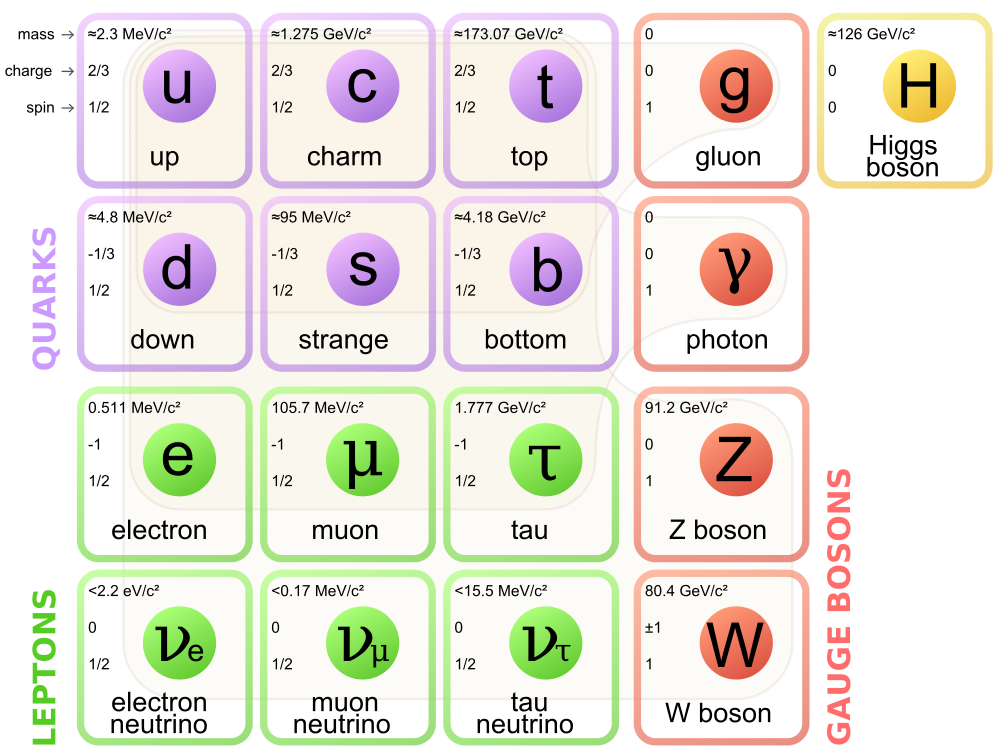
\includegraphics[width=.8\textwidth]{./figures/theory/standardmodel}
	\caption{Standard Model of elementary particle physics (from \korr{QUELLE: wiki})}
	\label{fig:standard_model}
\end{figure}

\subsection{Heavy Vector Boson Z$^0$}

The particle of interest for this experiment is the Z~boson \korr{dessen} decays are studied.
The Z~boson has a mass of \SI{91.2}{GeV} and a decay width of \SI{2.5}{GeV}.
It was discovered in 1983 in collider experiments at CERN.

\subsubsection{Decays of Z$^0$}

Z~bosons can decay in many different ways.
The final state of their decays can contain quarks, charged leptons and neutrinos, although it must be noted, that the top quark can not be produced since it is way heavier than the Z~boson.
Due to conservation laws the Z~boson may produce only pairs of particles and antiparticles (e.g. electron and positron or neutrino and corresponding antineutrino).
In case of production of a quark-antiquark pair the final state particles will form jets.
Because of confinement in QCD the strong interaction becomes stronger for larger distances between two strongly interacting particles.
If quark and antiquark fly apart a QCD field with high energy is created between them, where additional quark-antiquark pairs can be produced.
This process repeats itself as long as the particles have more energy than needed for formation of colourless hadrons.
As a result a hadronic decay of Z~bosons leads to a high number of final state particles, called jets.
Possible Feynman diagrams for the mentioned processes are shown in figure \korr{REF}.

\korr{BILD Feynman Diagramme}

\subsubsection{Forward-Backward Asymmetry A$_\mathrm{FB}$}

In a $e^+e^- \rightarrow f\bar{f}$ reaction the differential cross section of the produced fermions is different for the forward and backward hemispheres.
Those are defined by the angle $\theta$ between incoming positron and outgoing positively charged particle.
In this lab experiment, the asymmetry A$_\mathrm{FB}$ is measured in $e^+e^- \rightarrow \mu^+\mu^-$ events. 
\korr{hier noch ein paar von den schäbigen Formeln rausknallen?}

\subsection{The OPAL Experiment}

The OPAL~detector was used from 1989 to 2000 at the LEP storage ring at the CERN facility in Switzerland.
It was designed to detect all kinds of particles produced in collisions of electrons and positrons.
To cover most of the solid angle it had a barrel-like structure and consisted of a cylinder and two endcaps.
For tracking and vertex reconstruction purposes the inner part is formed by a semiconductor strip detector and multiple proportional chambers.
To measure the momentum of charged particles, the whole inner detector is surrounded by a solenoid which created a magnetic field.
The solenoid is followed by the calorimeters, first the electromagnetic and after that the hadronic one.
As a last layer muon chambers are installed which consist of a tracking detector themselves.
\korr{OPAL Bild?}

\section{Part I: Analysis of Event Displays}

On the first day the software \texttt{GROPE} was used to study event displays and detector responses of the OPAL detector.

\subsection{Part I: Analysis of Event Displays}

To learn how to distinguish the different decay channels of the Z boson test samples with events with only one decay mode have been investigated.
In the following part the measured properties of the observed events and exemplary pictures of the detector response are presented.

\subsubsection{Z$^0\rightarrow e^+e^-$}

A decay into electrons can easily be identified by the energy deposited in the electromagnetic calorimeters.
The final state particles are flying approximately in opposite direction and are ideally completely stopped in the calorimeter.
A track for every particle can be observed in the tracking chamber.
Additional hits in the electromagnetic calorimeters probably occur due to bremsstrahlung photons which leave no track in the inner detector.
\begin{sidewaystable}
	\centering
	\begin{tabular}{ccccccl}
	\toprule
	Run & Event & Ctrk(SumP) & Ctrk(N) & Ecal (SumE) & Hcal (SumE) & Comments \\
	\midrule
	2566 & 163733 & 50.9       & 2       & 82.6       & 0.0        &  not exactly back to back electrons, initial or final state radiation\\
	2566 & 165523 & 91.9       & 2       & 90.0       & 0.0        &  \\
	2566 & 165548 & 82.5       & 3       & 92.3       & 0.0        &  \\
	2566 & 165576 & 80.9       & 2       & 86.8       & 0.0        &  \\
	2566 & 166436 & 38.1       & 2       & 89.5       & 0.0        &  \korr{Bremsstrahlung?}\\
	2566 & 167987 & 83.8       & 2       & 87.5       & 0.0        &  \\
	2566 & 168389 & 87.4       & 2       & 93.2       & 0.0        &  \\
	2566 & 170045 & 69.3       & 2       & 90.7       & 0.0        &  \\
	2566 & 170379 & 86.1       & 2       & 89.4       & 0.5        &  \\
	2566 & 197594 & 90.3       & 2       & 90.6       & 0.0        &  \\
	2566 & 197889 & 92.1       & 2       & 88.5       & 0.5        &  \\
	2570 & 28178  & 81.7       & 3       & 91.6       & 0.0        &  third track starting at interaction point observable\\
	2570 & 28499  & 89.6       & 2       & 92.5       & 0.0        &  \\
	2570 & 28743  & 61.1       & 2       & 89.2       & 0.0        &  \korr{Bremsstrahlung?}\\
	2570 & 28777  & 88.4       & 3       & 89.1       & 0.0        &  third track present that follows a helix, probably $\delta$ electron\\
	2570 & 88224  & 90.9       & 2       & 90.5       & 0.3        &  \\
	2570 & 90060  & 64.6       & 2       & 88.8       & 0.0        &  \korr{Bremsstrahlung?}\\
	2570 & 91274  & 95.6       & 2       & 96.2       & 0.0        &  \\
	2571 & 418921 & 93.0       & 2       & 90.8       & 0.0        &  \\
	2571 & 420590 & 94.1       & 2       & 89.2       & 0.0        &  \\
	\bottomrule
\end{tabular}
	\caption{Collected data from the electron dataset. All values for energies and momenta in \si{GeV}.}
\end{sidewaystable}

\subsubsection{Z$^0\rightarrow \mu^+\mu^-$}

Muons are detected in the muon chambers which form the outermost part of the detector.
Since all other particles (except the non-detectable neutrinos) are stopped before reaching the muon chamber a signal there can -- neglecting noise hits -- be identified as a muon. 
In general, muons are also created in a back to back configuration and leave a track in the tracking detector.
\begin{sidewaystable}
	\centering
	\begin{tabular}{ccccccl}
	\toprule
	Run & Event & Ctrk(SumP) & Ctrk(N) & Ecal (SumE) & Hcal (SumE) & Comments \\
	\midrule
	2568 & 80617  & 90.1  & 2 & 1.6 & 7.0  &  \\ \midrule
	2568 & 84297  & 93.0  & 2 & 1.6 & 8.7  &  \\
	2568 & 85398  & 96.8  & 2 & 2.0 & 0.0  &  \\
	2568 & 87693  & 89.1  & 2 & 2.3 & 8.5  &  \\
	2568 & 89929  & 90.5  & 2 & 1.5 & 7.2  &  \\
	2568 & 91048  & 91.8  & 2 & 1.8 & 4.3  &  \\
	2568 & 92681  & 86.3  & 2 & 3.7 & 3.3  &  three hits, one could be cosmic, not coming from IP\\
	2568 & 93199  & 99.2  & 2 & 1.3 & 2.9  &  \\
	2568 & 95202  & 88.2  & 2 & 1.6 & 3.0  &  \\
	2568 & 99962  & 90.9  & 2 & 1.3 & 6.7  &  \\
	2568 & 100566 & 95.6  & 2 & 2.5 & 6.1  &  \\
	2568 & 100721 & 75.3  & 2 & 3.1 & 6.8  &  bent track due to initial state radiation \\
	2568 & 102167 & 85.2  & 2 & 5.8 & 4.4  &  \\
	2568 & 105720 & 98.6  & 2 & 3.6 & 5.7  &  \\
	2568 & 106346 & 86.8  & 2 & 1.9 & 7.9  &  \\
	2568 & 107030 & 98.0  & 2 & 1.9 & 2.0  &  \\
	2568 & 107772 & 108.3 & 2 & 2.0 & 8.5  &  one of the muons created two hits, three muon hits in total\\
	2568 & 108553 & 92.4  & 2 & 3.6 & 6.7  &  \\
	2568 & 110610 & 92.0  & 2 & 1.9 & 22.6 & \korr{Warum soviel Hcal? Kann man das erklären?} \\
	2570 & 29023  & 92.6  & 2 & 3.6 & 5.7  &  \\
	\bottomrule
\end{tabular}
	\caption{Collected data from the muon dataset. All values for energies and momenta in \si{GeV}.}
\end{sidewaystable}

\subsubsection{Z$^0\rightarrow \tau^+\tau^-$}

Because of the short lifetime of the $\tau$ lepton it can not be detected directly but by its decay products.
Because it can decay in both leptons and hadrons there are two possible types of detector responses.
In a leptonic $\tau$ decay an electron or muon and two neutrinos are created and seen as charged tracks in the inner detector.
They cause signals either in the electromagnetic calorimeter or in the muon chambers while the neutrinos are not detected.

In a hadronic $\tau$ decay a neutrino and hadrons are produced.
All hadrons create a shower in the hadronic calorimeter but depending on their charge a track can not always be observed.
\begin{sidewaystable}
	\centering
	\resizebox{\textwidth}{!}{
		\begin{tabular}{ccccccll}
	\toprule
	Run & Event & Ctrk(SumP) & Ctrk(N) & Ecal (SumE) & Hcal (SumE) & Decay & Comments \\
	\midrule
	2566 & 170371 & 74.0 & 5 & 51.1 & 10.2 & 3 $\pi^\pm$, 1 $\pi^\pm$ & 3 and 1 prong \\
	2566 & 170508 & 46.5 & 2 & 17.3 & 8.2  & 1 $\pi^\pm$, 1 $\mu^\pm$ & 1 and 1 prong \\
	2566 & 179750 & 30.8 & 2 & 1.6  & 6.3  & 2 $\mu^\pm$ & 1 and 1 prong  \\
	2566 & 184010 & 29.5 & 2 & 10.2 & 4.1  & 1 $\mu^\pm$, 1 $e^\pm$ & 1 and 1 prong  \\
	2566 & 184435 & 33.1 & 2 & 1.5  & 10.6 & 2 $\mu^\pm$ & 1 and 1 prong  \\
	2566 & 189056 & 24.4 & 2 & 12.4 & 11.7 & 1 $e\pm$, 1 $\pi^\pm$ & 1 and 1 prong \\
	2566 & 208314 & 36.0 & 4 & 16.1 & 5.7  & 1 $\mu^\pm$, 3 $\pi^\pm$ & 1 and 3 prong  \\
	2566 & 212745 & 41.3 & 2 & 11.1 & 20.0 & 1 $e^\pm$, 1 $\mu^\pm$ & 1 and 1 prong \\
	2570 & 29664  & 49.7 & 2 & 5.2  & 20.3 & 2 $\mu^\pm$ & 1 and 1 prong, additional muon, probably cosmic background \\
	2570 & 30348  & 33.4 & 2 & 23.6 & 6.9  & 1 $e^\pm$, 1 $\mu^\pm$ & 1 and 1 prong  \\
	2570 & 34612  & 14.1 & 2 & 3.3  & 6.3  & 1 $\mu^\pm$, 1 $\pi^\pm$ & 1 and 1 prong  \\
	2570 & 39992  & 19.7 & 2 & 15.9 & 3.8  & 1 $e\pm$, 1 $\pi^\pm$ & 1 and 1 prong \\
	2570 & 42200  & 26.8 & 2 & 16.5 & 3.4  & 1 $\mu^\pm$, 1 $e^\pm$ & 1 and 1 prong \\
	2570 & 45609  & 23.4 & 5 & 27.0 & 17.1 & 1 $\mu^\pm$, 1 $\pi^\pm$ & 1 and 1 prong, one additional conversion photon \\
	2570 & 47033  & 23.8 & 2 & 29.4 & 3.6  & 2 $e^\pm$ & 1 and 1 prong \\
	2572 & 98915  & 39.0 & 2 & 18.9 & 4.4  & 1 $\mu^\pm$, 1 $e^\pm$ & 1 and 1 prong \\
	2572 & 102412 & 24.1 & 2 & 46.5 & 7.3  & 1 $e\pm$, 1 $\pi^\pm$ & 1 and 1 prong \\
	2572 & 102586 & 38.5 & 5 & 28.5 & 0.0  & 1 $e^\pm$, 3 $\pi^\pm$ & 1 and 3 prong, possible additional cosmic radiation \\
	2572 & 108411 & 35.3 & 2 & 51.8 & 2.3  & 2 $\pi^\pm$ & 1 and 1 prong, additional $\pi^0$ decaying to photon \\
	2572 & 109621 & 17.8 & 2 & 2.5  & 5.0  & 2 $\mu^\pm$ & 1 and 1 prong, in total four muon hits due to cosmic background \\
	\bottomrule
\end{tabular}
	}
	\caption{Collected data from the tau dataset. All values for energies and momenta in \si{GeV}. To identify the decay, only the charged particles are given. There are always neutrinos present which can not be detected and often times it is possible to have $\pi^0$ mesons that interact electromagnetically.}
\end{sidewaystable}

\subsubsection{Z$^0\rightarrow q\bar{q}$}

Decays of Z$^0$ into quark-antiquark pairs always produce jets where quarks hadronize to mesons or baryons.
Those can be identified as a large number of charged tracks in the tracking system.
In addition some of the hadrons decay into leptons which can be seen as signal in the electromagnetic calorimeter or the muon chambers.
The hadrons are stopped and seen as showers in the hadronic calorimeter.
\begin{table}[h]
	\centering
	\resizebox{\textwidth}{!}{
		\begin{tabular}{S[table-format=4.0]S[table-format=6.0]S[table-format=2.1]S[table-format=2.0]S[table-format=2.1]S[table-format=2.1]l}
	\toprule
	{Run} & {Event} & {\texttt{Ctrk(Sump)}} & {\texttt{Ctrk(N)}} & {\texttt{Ecal(SumE)}} & {\texttt{Hcal(SumE)}} & {Comments} \\
	\midrule
	2566 & 164184 & 37.7 & 15 & 37.0   & 14.1 & two jets with one muon each \\
	2566 & 195995 & 39.2 & 17 & 66.8 & 9.9  &  \\
	2566 & 196117 & 64.6 & 46 & 53.0   & 13.0   & low momentum particles on helical track \\
	2566 & 196548 & 33.3 & 8  & 67.5 & 13.3 & two jets with one muon each \\
	2568 & 78191  & 45.3 & 36 & 53.2 & 7.7  & \\
	2568 & 78425  & 59.9 & 41 & 53.2 & 13.8 & \\
	2568 & 78553  & 21.9 & 9  & 65.2 & 8.8  & \\
	2568 & 78787  & 55.9 & 16 & 50.4 & 24.3 & one jet containing a muon \\
	2568 & 79038  & 38.1 & 30 & 68.3 & 13.8 & three jets \\
	2568 & 79043  & 34.4 & 22 & 75.5 & 6.2  & \\
	2568 & 79181  & 51.2 & 36 & 62.3 & 5.5  & \\
	2568 & 79337  & 63.1 & 23 & 56.0   & 17.2 & \\
	2568 & 79487  & 59.0   & 23 & 60.6 & 8.5  & one jet containing a muon \\
	2568 & 79517  & 62.2 & 26 & 67.2 & 20.4 &  \\
	2568 & 79642  & 43.3 & 30 & 71.7 & 4.3  & three jets  \\
	2570 & 88252  & 47.8 & 40 & 61.4 & 5.7  & two jets with one muon each \\
	2570 & 88262  & 67.9 & 19 & 52.1 & 10.6 &  \\
	2570 & 88303  & 52.1 & 14 & 61.0   & 4.4  & \\
	2570 & 88328  & 82.6 & 29 & 53.8 & 16.4 & \\
	\bottomrule
\end{tabular}
	}
	\caption{Collected data from the hadronic dataset. All values for energies and momenta in \si{GeV}.}
\end{table}

\subsubsection{Event Identification in Test Sample}

Based on the observations from the previous exercise it was possible to evaluate cuts to apply on the data in order to distinguish between different decay channels of the Z boson.
The used cuts are given in table \ref{tab:cut_criteria_day1} and could be reviewed by looking on the events in a test sample.
All of the decay channels found with the cut criteria could be verified by analysis of event displays.
\begin{table}[h]
	\centering
	\begin{tabular}{lcccc}
	\toprule
	 & $e$ & $\mu$ & $\tau$ & hadrons \\
	 \midrule
	\texttt{ncharged} & $< 5$  & $< 4$  & $< 8$ & $\geq 8$ \\
	\texttt{pcharged} & $> 30$ & $> 55$ & $>1\,\land\,<75$ & --\\
	\texttt{e\_ecal}  & $> 70$ & $< 15$  & $< 75$ & $> 20$ \\
	\texttt{e\_hcal}  & $< 15$  & $< 25$ & -- & -- \\
	\bottomrule
\end{tabular}
	\caption{Applied cuts on the data to identify the decay channel.}
	\label{tab:cut_criteria_day1}
\end{table}
\begin{table}[h]
	\centering
	\resizebox{\textwidth}{!}{
		\begin{tabular}{S[table-format=4.0]S[table-format=5.0]S[table-format=2.1]S[table-format=2.0]S[table-format=2.1]S[table-format=2.1]ll}
	\toprule
	{Run} & {Event} & {\texttt{Ctrk(Sump)}} & {\texttt{Ctrk(N)}} & {\texttt{Ecal(SumE)}} & {\texttt{Hcal(SumE)}} & ident.\ decay & Comments \\
	\midrule
4353 & 1080  & 39.5 & 19 & 44.3 & 15.6 & hadronic 		& two jets with one muon each \\
4353 & 2387  & 42.8 & 36 & 57.1 & 12.5 & hadronic 		& jets and one muon \\
4353 & 5386  & 95.7 & 2  & 93.4 & 0.0  & $e^+e^-$ 		& \\
4353 & 6057  & 90.8 & 2  & 1.4  & 4.1  & $\mu^+\mu^-$ 	& \\
4353 & 6696  & 36.5 & 4  & 35.8 & 10.8 & $\tau^+\tau^-$ & 1 and 3 prong \\
4353 & 7137  & 97.0 & 2  & 2.2  & 8.9  & $\mu^+\mu^-$   & possible cosmic background muon \\
4353 & 7219  & 42.9 & 68 & 48.5 & 6.2  & hadronic 		& \\
4353 & 8323  & 35.0 & 5  & 40.8 & 3.3  & $\tau^+\tau^-$ & muon and 3 prong, probably wrong reconstruction \\
4353 & 8641  & 75.8 & 21 & 45.8 & 21.0 & hadronic 		& two jets                                         \\
4353 & 9149  & 95.2 & 2  & 1.3  & 7.9  & $\mu^+\mu^-$   &                                                   \\
4353 & 9289  & 22.7 & 2  & 34.4 & 0.0  & $\tau^+\tau^-$ & 1 and 1 prong, considerable missing energy due to $\nu$\\
4353 & 9593  & 44.3 & 4  & 37.8 & 2.6  & $\tau^+\tau^-$ & 1 and 3 prong                                              \\
4353 & 9880  & 53.1 & 21 & 36.2 & 22.9 & hadronic 		&                                                   \\
4353 & 10900 & 89.5 & 2  & 92.0 & 0.0  & $e^+e^-$   	&                                                   \\
4353 & 11844 & 89.1 & 2  & 89.7 & 0.0  & $e^+e^-$    	&                                                   \\
4353 & 13556 & 4.1  & 2  & 4.4  & 0.0  & $\tau^+\tau^-$ & two-photon reaction (misidentification) \\
4353 & 14063 & 87.8 & 2  & 1.4  & 4.3  & $\mu^+\mu^-$   & \\
4353 & 14640 & 75.3 & 2  & 90.0 & 0.0  & $e^+e^-$    	& additional radiation losses \\
4353 & 14744 & 93.7 & 2  & 1.6  & 6.8  & $\mu^+\mu^-$   & \\
4353 & 15775 & 67.1 & 2  & 93.6 & 0.0  & $e^+e^-$    	& additional radiation losses \\
	\bottomrule
\end{tabular}
	}
	\caption{Collected data from the events in the test sample dataset. All values for energies and momenta in \si{GeV}.}
\end{table}

\clearpage
\section{Part II: Statistical Analysis of $\mathrm{Z}^0$ Decays}

\subsubsection{Variables and Cut Optimization}
The second part of the experiment is performed using the data analysis software \texttt{PAW}.
To accustom ourselves with \texttt{PAW}, several variables from different Monte-Carlo simulated datasets have been plotted.
When displaying \texttt{pcharged} one maximum at~\SI{0}{GeV} in the electron and muon data could be observed.
To investigate the source for this observation, additional cuts on other variables have been set until it was found that those events come from particles that have been detected at a very small angle with respect to the beam axis.
Because of the bad sensitivity in these regions the data were cut on the angle such that $\left|\cos\theta\right|<\num{0.9}$.
It must be noted that this cut has to be used for all of the following tasks.

\subsubsection{Separating s- and t-channel}

\subsubsection{Cuts for Event Selection}

In order to optimize the cuts for event identification the variables \texttt{ncharged}, \texttt{pcharged}, \texttt{e\_ecal}, \texttt{e\_hcal} have been plotted as histograms for all datasets.
Baed on the observed distributions cuts on the parameters have been set such that we can determine the decay channel in good approximation by cutting the data.
The resulting histograms are shown in figures \korr{REF} where one cut for identifying one decay channel has been applied to all datasets in each figure.
\korr{FIGURES}
While retaining as much events as possible it was not possible to fully differentiate between the decay channels.
Because of this, there are some misinterpreted events for datasets which do not correspond to the applied cuts.
For identifying electrons an additional cut on the angle was set such that only s-channel electrons are selected.
An overview of the cuts is given in table \ref{tab:cut_criteria}.
\begin{table}[h]
	\centering
	\begin{tabular}{lcccc}
	\toprule
	 & $e$ & $\mu$ & $\tau$ & hadrons \\
	 \midrule
	\texttt{ncharged} & $< 5$  & $< 4$  & $< 8$ & $\geq 8$ \\
	\texttt{pcharged} & $> 30$ & $> 55$ & $>1\,\land\,<75$ & --\\
	\texttt{e\_ecal}  & $> 70$ & $< 15$  & $< 75$ & $> 20$ \\
	\texttt{e\_hcal}  & $< 15$  & $< 25$ & -- & -- \\
	\bottomrule
\end{tabular}
	\caption{Applied cuts on the data to identify the decay channel. An additional cut on the angle is used for electrons since only the s-channel is of interest.}
	\label{tab:cut_criteria}
\end{table}

\subsubsection{Efficiency Matrix}

Obviously one loses events in setting cuts on the data which makes it necessary to analyse the efficiency, i.e. the fractional losses of these cuts.
Knowing that each of the datasets have been simulated with \num{100000} events the efficiency can be calculated from the number of remaining events that fulfill the cut conditions.
A matrix formalism can be used to describe the number of measured events per decay channel $\vec{N}_\mathrm{meas}=(e_\mathrm{meas}, \mu_\mathrm{meas}, \tau_\mathrm{meas}, q_\mathrm{meas})^T$ by the number of events that have been simulated in this channel $\vec{N}_\mathrm{orig}$:
\begin{align}
\vec{N}_\mathrm{meas} = A \cdot \vec{N}_\mathrm{orig}
\end{align}
The values of $A$ describe how many events of one decay channel are identified as such or as one of the other decay channels.
With the measured event numbers after applying the cuts on all datasets, $A$ is then given by
\begin{align}
A = \begin{pmatrix}
	x & \dots \\
	\vdots & \ddots \\
	\end{pmatrix}
\end{align}

\subsubsection{Determination of the Differential Cross Sections}

\subsubsection{Determination of the Forward-Backward Asymmetry using Muons}

\subsubsection{Fitting Resonance Curves}

\subsubsection{Calculation of the Partial Widths}

\subsubsection{Lepton Universality}

\subsubsection{Number of Light Neutrino Generations}

\subsubsection{Discussion of Uncertainties}

\subsection{Stuff}

Correction for missing s-channel electrons:
\begin{align*}
\frac{\int_{-1}^{1}(1 + \cos^2\theta) \dinf{\cos\theta}}{\int_{-0.9}^{0.5}(1 + \cos^2\theta) \dinf{\cos\theta}} = 1.5829
\end{align*}


Variance of the binomial distribution:
\begin{align*}
	\mathrm{Var} = n p (1 - p) 
\end{align*}


Calculation of the cross section
\begin{align*}
	N &= \sigma \cdot \int \mathcal{L} \dinf{t}\\
	\sigma &= \frac{N}{\int \mathcal{L} \dinf{t}}
\end{align*}

\section{Conclusion}


\FloatBarrier
% BIBLIOGRAPHIE
\vspace{\fill}
% Maximale Anzahl der Einträge in Klammer
% Zitieren mit \cite{lamport94}
\begin{thebibliography}{19}
\bibitem{steck}
D.\ A.\ Steck,
\emph{Rubidium 85 D Line Data},
\url{http://steck.us/alkalidata} (Revision 2.1.6, 20.\ September 2013)

\bibitem{script}
Skript zum Versuch,
\emph{FP Experiment: Rubidium MOT},
(Stand: Januar 2014).
	
\bibitem{anleitung}
	\emph{Advanced Laboratory Course (physics601): Description of Experiments}, BONN-AT-2016-01MP, Universität Bonn, Januar 2016
	
\bibitem{foot}
C.\ J.\ Foot,
\emph{Atomic Physics},
Oxford University Press, 2005.

\bibitem{wieman}
	C.\ Wieman, G.\ Flowers, S.\ Gilbert,
	\emph{Inexpensive laser cooling and trapping experiment for undergraduate laboratories},
	Am.\ J.\ Phys.\ \textbf{63} (4), April 1995.

\bibitem{handbook_spectroscopic_data}
	J.\ E.\ Sansonetti, W.\ C.\ Martin,
	\emph{Handbook of Basic Atomic Spectroscopic Data},
	National Institute of Standards and Technology (NIST), \url{http://physics.nist.gov/PhysRefData/Handbook/Tables/rubidiumtable1.htm} (Letzter Aufruf: 7.\ April 2016).

\bibitem{force_in_mot}
	A.\ M.\ Steane, M.\ Chowdhury, C.\ J.\ Foot,
	\emph{Radiation force in the magneto-optical trap},
	J.\ Opt.\ Soc.\ Am.\ B \textbf{9}, 2142 (1992).
\end{thebibliography}

% APPENDIX
\begin{appendix}
\newpage
\section{Appendix}
\end{appendix}

\end{document}
